% rf_shot_tx.tex — ONE source, ONE rendered SVG (rf_shot_tx.svg), embedded in
% ../rfshotbuf/tx.md.
%
% The claim: a shot transmitter is three things and one memory between them.  A host hands a header
% and its samples in on ONE stream and gets ONE verdict back; the loader writes them to a memory; the
% player reads that memory at the converter's pace.  The lock the two tasks use to hand the memory
% over is DELIBERATELY ABSENT — it is how the design works, not what a user has to know, and it lives
% in ../rfshotbuf/tx_internal.md.
%
% Render: bash render.sh   (MiKTeX pdflatex -> PDF -> dvisvgm --pdf -> SVG)
\documentclass[tikz,border=4pt]{standalone}
\usepackage{tikz}
\usetikzlibrary{arrows.meta,positioning,calc,fit,backgrounds}

% Theme-neutral palette, same as rf_domains.tex: the SVG is viewed on both light and dark docs pages,
% so fills stay pale and every stroke and label is explicit rather than inherited.
\definecolor{hostfill}{HTML}{ECE4F2}
\definecolor{hostline}{HTML}{6B4E8F}
\definecolor{taskfill}{HTML}{DCE9F7}
\definecolor{taskline}{HTML}{2C6FB5}
\definecolor{memfill}{HTML}{F2E6D0}
\definecolor{memline}{HTML}{9A6B1F}
\definecolor{cnvfill}{HTML}{E8F0E4}
\definecolor{cnvline}{HTML}{4F7A3F}
\definecolor{inkgray}{HTML}{444444}

\begin{document}
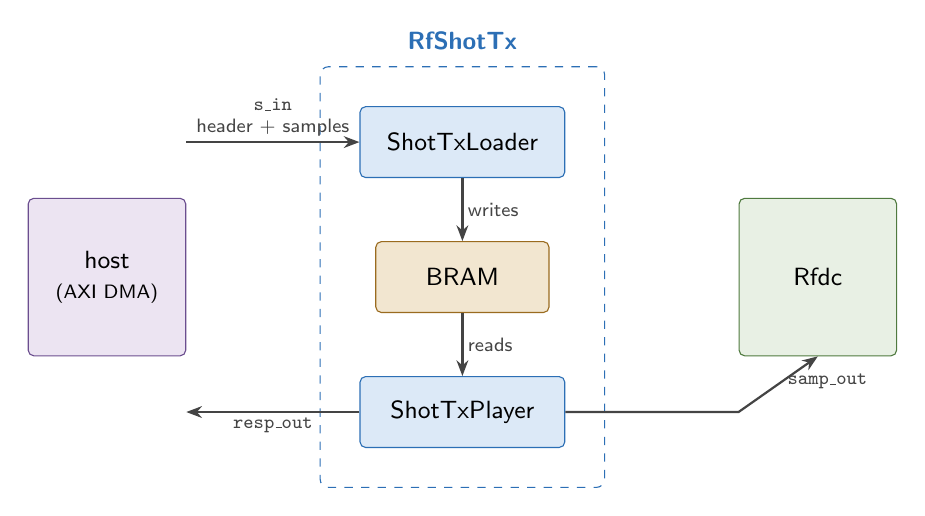
\begin{tikzpicture}[
  font=\sffamily\small,
  host/.style = {draw=hostline, fill=hostfill, rounded corners=2pt,
                 minimum width=20mm, minimum height=20mm, align=center},
  task/.style = {draw=taskline, fill=taskfill, rounded corners=2pt,
                 minimum width=26mm, minimum height=9mm},
  mem/.style  = {draw=memline, fill=memfill, rounded corners=2pt,
                 minimum width=22mm, minimum height=9mm},
  cnv/.style  = {draw=cnvline, fill=cnvfill, rounded corners=2pt,
                 minimum width=20mm, minimum height=20mm, align=center},
  ln/.style   = {-{Stealth[length=2mm]}, draw=inkgray, thick},
  lbl/.style  = {font=\sffamily\scriptsize, text=inkgray, inner sep=1.6pt},
]

% --- the column of three, and the memory between the two tasks -----------------------------------
\node[task]                        (load) {ShotTxLoader};
\node[mem,  below=8mm of load]     (bram) {BRAM};
\node[task, below=8mm of bram]     (play) {ShotTxPlayer};

\node[host, left=24mm of bram]     (hostn) {host\\{\scriptsize(AXI DMA)}};
\node[cnv,  right=24mm of bram]    (rfdc)  {Rfdc};

% --- in, and the verdict back ---------------------------------------------------------------------
\draw[ln] (hostn.east |- load) -- node[lbl, above, align=center]
          {\texttt{s\_in}\\header + samples} (load.west);
\draw[ln] (load.west |- play) -- node[lbl, below] {\texttt{resp\_out}} (hostn.east |- play);

% --- through the memory ----------------------------------------------------------------------------
\draw[ln] (load.south) -- node[lbl, right] {writes} (bram.north);
\draw[ln] (bram.south) -- node[lbl, right] {reads}  (play.north);

% --- out to the converter --------------------------------------------------------------------------
\draw[ln] (play.east) -- ($(rfdc.west |- play)$) -- node[lbl, right, pos=0.55]
          {\texttt{samp\_out}} (rfdc.south);

% --- the design scope --------------------------------------------------------------------------------
\begin{scope}[on background layer]
  \node[draw=taskline, dashed, rounded corners=3pt, inner sep=5mm,
        fit=(load)(bram)(play)] (scope) {};
\end{scope}
\node[lbl, above=1.5mm of scope.north, text=taskline, font=\sffamily\small\bfseries] {RfShotTx};

\end{tikzpicture}
\end{document}
